% !TeX root = RJwrapper.tex
\title{Concise indicator variable recoding with ind2cat}
\author{by Evangeline Reynolds}

\maketitle

\abstract{%
Indicator variables are often used in data analyses given the ease which
with they are created, stored and interpreted. They concisely encode
information about the presence or not of a condition for observational
units. The variable name encapsulates the information about the true
condition, the variable's values (TRUE and FALSE, 1 or 0, ``Yes'' or
``No''), indicate if the condition is true for the observational unit.
When using indicator variables to use in summary products, analysts
often make a choice between using an indicator variable as-is or
crafting categorical variables where values can be directly interpreted.
Using the indicator variable as-is may be motivated by time savings.
\{\{ind2cat\}\} can help analysts concisely translate indicator
variables to categorical variables for reporting products, yielding more
polished outputs even in the exploratory analysis stage. By default,
ind2cat creates the categorical variable from the indicator variable
name, resulting in a light weight syntax.
}

\begin{enumerate}
\def\labelenumi{\arabic{enumi})}
\tightlist
\item
  Is there already a solution
\item
  unsure if there are fundamental problems with this approach
\end{enumerate}

\hypertarget{some-things-to-move-ind2cat-out-of-proof-of-concept-phase}{%
\subsection{Some things to move ind2cat out of proof of concept
phase}\label{some-things-to-move-ind2cat-out-of-proof-of-concept-phase}}

\begin{itemize}
\tightlist
\item
  change to Rlang for grabbing function name (Claus Wilke)
\item
  left join instead of ifelse to make code more performant (Emily
  Rederer)
\item
  make ``Y'' ``N'' a lot stricter - right now we're assuming a ton!
  Danger.
\end{itemize}

\hypertarget{introduction}{%
\section{Introduction}\label{introduction}}

Recoding indicator variable values to meaningful and appropriately
ordered categories often involves redundancy.

\emph{more description of example here}

\begin{Schunk}
\begin{Sinput}
library(tidyverse)

data.frame(ind_graduated = c(T,T,F)) |>
  mutate(cat_graduated  = ifelse(ind_graduated, 
                                 "graduated", 
                                 "not graduated")) |>
  mutate(cat_graduated = fct_rev(cat_graduated))  
\end{Sinput}
\begin{Soutput}
       ind_graduated cat_graduated
     1          TRUE     graduated
     2          TRUE     graduated
     3         FALSE not graduated
\end{Soutput}
\end{Schunk}

ind2cat's ind\_recode function avoids repetition by creating categories
based on the indicator variable name. Using the the function
ind\_recode(), we can accomplish the same task shown above more
succinctly:

\begin{Schunk}
\begin{Sinput}
library(ind2cat)

data.frame(ind_graduated = c(T,T,F)) |>
  mutate(cat_graduated  = ind_recode(ind_graduated))
\end{Sinput}
\begin{Soutput}
       ind_graduated cat_graduated
     1          TRUE     graduated
     2          TRUE     graduated
     3         FALSE not graduated
\end{Soutput}
\end{Schunk}

Furthermore, ind\_recode's functionality allows analysts to move from a
first-cut recode that delivers meaningful categories to fully customized
categories.

\begin{Schunk}
\begin{Sinput}
data.frame(ind_graduated = c(T,T,F)) %>% 
  mutate(cat_graduated  = ind_recode(ind_graduated, 
                                     cat_false = "current"))
\end{Sinput}
\begin{Soutput}
       ind_graduated cat_graduated
     1          TRUE     graduated
     2          TRUE     graduated
     3         FALSE       current
\end{Soutput}
\end{Schunk}

\hypertarget{status-quo-analysts-make-a-choice-between-directly-using-indicators-or-verbose-recode}{%
\section{Status-Quo: Analysts make a choice between directly using
indicators or verbose
recode}\label{status-quo-analysts-make-a-choice-between-directly-using-indicators-or-verbose-recode}}

\hypertarget{current-proceedures-for-recoding-indicator-variables-to-a-categorial-variable-is-inelegant.}{%
\subsection{Current proceedures for recoding indicator variables to a
categorial variable is
inelegant.}\label{current-proceedures-for-recoding-indicator-variables-to-a-categorial-variable-is-inelegant.}}

Current methods for recoding indicator variables is repetitive and
verbose, as shown in the examples that follow.

\begin{Schunk}
\begin{Sinput}
tidytitanic::passengers %>% 
  tibble() %>% 
  mutate(cat_survived = ifelse(survived, "survived", "not survived"), 
         .before = 1)
\end{Sinput}
\begin{Soutput}
     # A tibble: 1,313 x 6
        cat_survived name                                   class   age sex   survi~1
        <chr>        <chr>                                  <chr> <dbl> <chr>   <int>
      1 survived     Allen, Miss Elisabeth Walton           1st   29    fema~       1
      2 not survived Allison, Miss Helen Loraine            1st    2    fema~       0
      3 not survived Allison, Mr Hudson Joshua Creighton    1st   30    male        0
      4 not survived Allison, Mrs Hudson JC (Bessie Waldo ~ 1st   25    fema~       0
      5 survived     Allison, Master Hudson Trevor          1st    0.92 male        1
      6 survived     Anderson, Mr Harry                     1st   47    male        1
      7 survived     Andrews, Miss Kornelia Theodosia       1st   63    fema~       1
      8 not survived Andrews, Mr Thomas, jr                 1st   39    male        0
      9 survived     Appleton, Mrs Edward Dale (Charlotte ~ 1st   58    fema~       1
     10 not survived Artagaveytia, Mr Ramon                 1st   71    male        0
     # ... with 1,303 more rows, and abbreviated variable name 1: survived
\end{Soutput}
\begin{Sinput}
tidytitanic::passengers %>% 
ggplot() + 
  aes(x = sex) + 
  geom_bar() + 
  facet_grid(~ ifelse(survived, "survived", "not survived")) 
\end{Sinput}

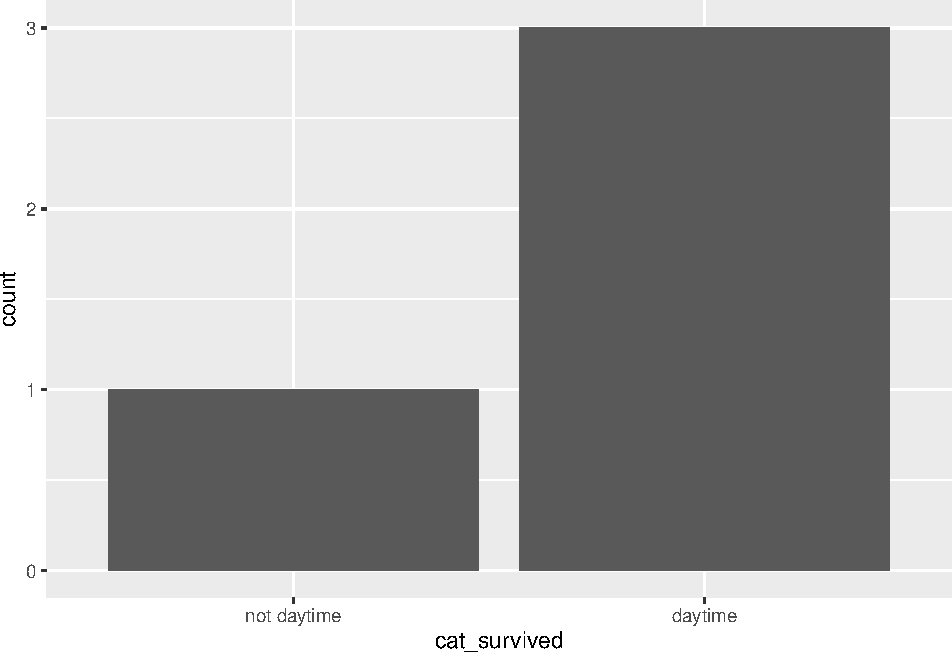
\includegraphics[width=0.69\linewidth]{r_journal_files/figure-latex/unnamed-chunk-4-1} \end{Schunk}

This solution above also does not address category display ordering;
ordering in products will be alphabetical and not reflect the F/T order
of the source variable. An additional step to reflect the source
variable, using a function like forcats::fct\_rev, may be required for
consistency in reporting.

\begin{Schunk}
\begin{Sinput}
data.frame(ind_daytime = c(T, F, T, T)) %>% 
    mutate(cat_survived = ifelse(ind_daytime, "daytime", "not daytime")) %>% 
  mutate(cat_survived = fct_rev(cat_survived)) %>% 
  ggplot() + 
  aes(x = cat_survived) + 
  geom_bar()
\end{Sinput}

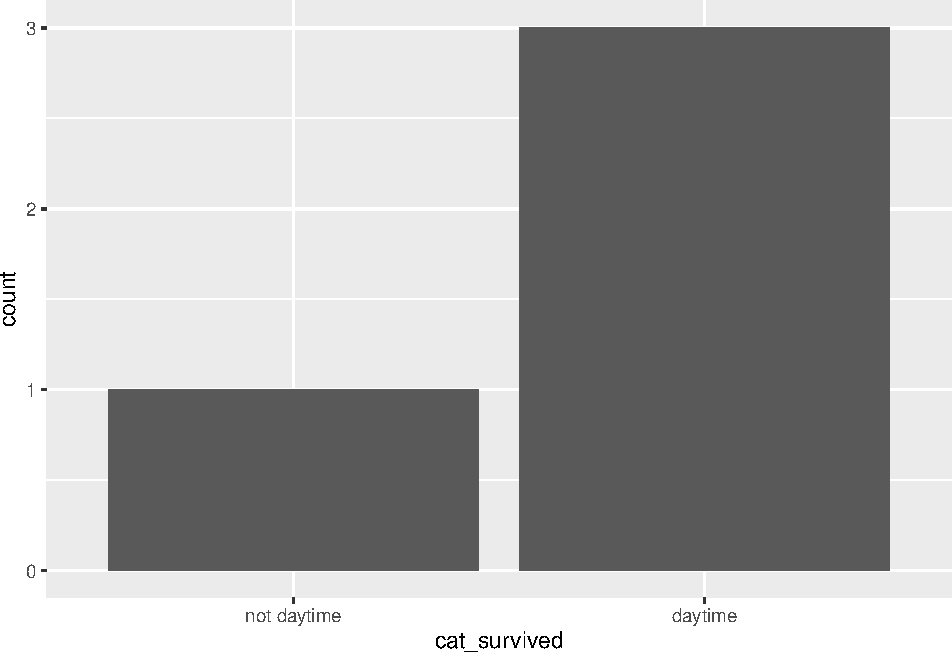
\includegraphics[width=0.69\linewidth]{r_journal_files/figure-latex/unnamed-chunk-5-1} \end{Schunk}

\hypertarget{direct-use-of-indicator-variables-in-data-products-makes-product-more-difficult-or-impossible-to-interpret.}{%
\subsection{Direct use of indicator variables in data products makes
product more difficult or impossible to
interpret.}\label{direct-use-of-indicator-variables-in-data-products-makes-product-more-difficult-or-impossible-to-interpret.}}

Given how verbose recoding can be, analyst may choose to forego a
recoding the variable, especially in exploratory analysis.

When indicator variables are not translated to a categorical analogue in
creating data products like tables and visuals, information is often
awkwardly displayed and is sometimes lost. When creating tables, using
an indicator variable directly can be awkward or insufficient for
interpretation.

Below, the column header from variable name and 0-1 categories preserves
information but is awkward:

\begin{Schunk}
\begin{Sinput}
tidytitanic::passengers %>% 
  count(survived) 
\end{Sinput}
\begin{Soutput}
       survived   n
     1        0 863
     2        1 450
\end{Soutput}
\end{Schunk}

In the following two-way table, information is completely lost:

\begin{Schunk}
\begin{Sinput}
tidytitanic::passengers %>% 
  janitor::tabyl(sex, survived) %>% 
  knitr::kable(caption = "C. ", format = kabel_format)
\end{Sinput}
\begin{table}

\caption{\label{tab:unnamed-chunk-7}C. }
\centering
\begin{tabular}[t]{l|r|r}
\hline
sex & 0 & 1\\
\hline
female & 154 & 308\\
\hline
male & 709 & 142\\
\hline
\end{tabular}
\end{table}

\end{Schunk}

Furthermore in creating ba

\begin{Schunk}
\begin{Sinput}
library(tidyverse)

tidytitanic::passengers %>% 
  ggplot() + 
  aes(x = survived) + 
  geom_bar()
\end{Sinput}
\begin{figure}
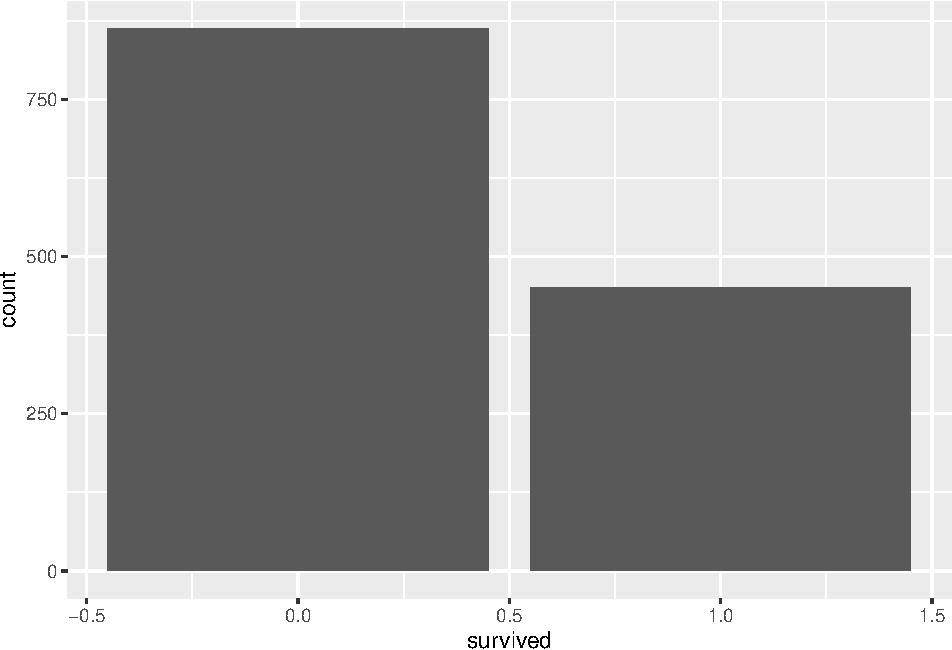
\includegraphics[width=0.69\linewidth]{r_journal_files/figure-latex/cars-1} \caption[A]{A. Bar labels + axis label preserves information but is awkward}\label{fig:cars}
\end{figure}
\end{Schunk}

\begin{Schunk}
\begin{Sinput}
tidytitanic::passengers %>% 
ggplot() + 
  aes(x = sex) + 
  geom_bar() + 
  facet_grid(~ survived)
\end{Sinput}
\begin{figure}
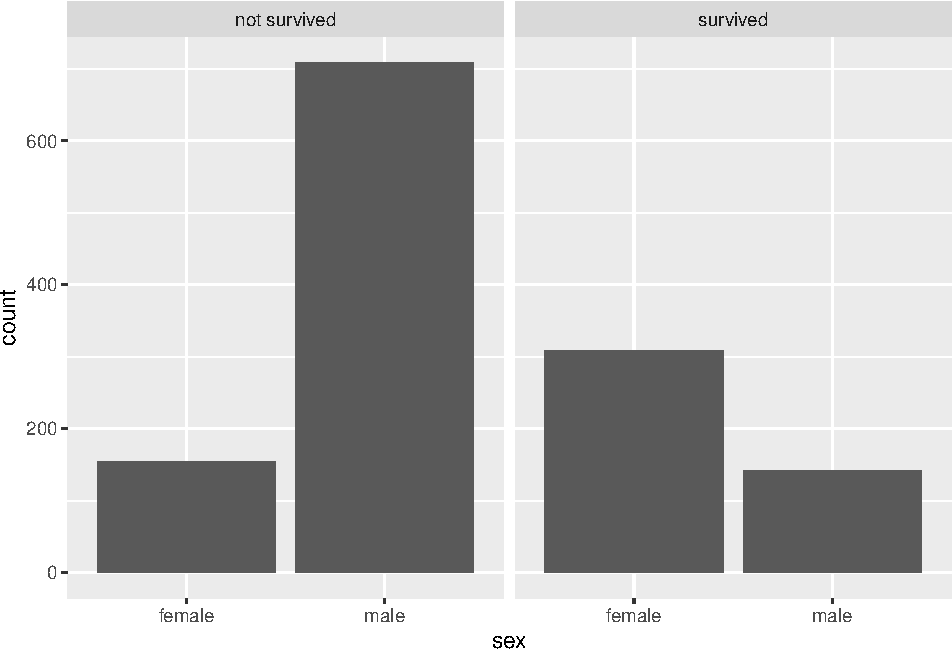
\includegraphics[width=0.69\linewidth]{r_journal_files/figure-latex/unnamed-chunk-8-1} \caption[D]{D. Facetting directly on an indicator variable with popular ggplot2 results in information loss}\label{fig:unnamed-chunk-8}
\end{figure}
\end{Schunk}

\hypertarget{introducing-ind_recode-ind_recode-function-uses-variable-name-as-starting-point-for-human-readable-categories}{%
\section{\texorpdfstring{Introducing ind\_recode \emph{ind\_recode()
function uses variable name as starting point for human-readable
categories}}{Introducing ind\_recode ind\_recode() function uses variable name as starting point for human-readable categories}}\label{introducing-ind_recode-ind_recode-function-uses-variable-name-as-starting-point-for-human-readable-categories}}

\begin{Schunk}
\begin{Sinput}
#' ind_recode
#'
#' @param var the name of an indicator variable
#' @param var_prefix a character string that will be ignored when creating the categorical variable
#' @param negator a character string used to create cat_false when cat_false is NULL, default is 'not'
#' @param cat_true a character string string to be used place of  T/1/"Yes" for the categorical variable output, if NULL the category is automatically generated from the variable name
#' @param cat_false a character string string to be used place of  F/0/"No" for the categorical variable output, if NULL the category is automatically generated from the cat true and the negator
#' @param rev logical indicating if the order should be reversed from the F/T ordering of the indicator source variable, default is FALSE
#'
#' @return
#' @export
#'
#' @examples
#' library(tibble)
#' library(dplyr)
#' tibble(ind_grad = c(0,0,1,1,1 ,0 ,0)) %>%
#'   mutate(cat_grad  = ind_recode(ind_grad))
#'
#' tibble(ind_grad = c(TRUE,TRUE,FALSE)) %>%
#'   mutate(cat_grad  = ind_recode(ind_grad))
#'
#' tibble(ind_grad = c("Y", "N")) %>%
#'   mutate(cat_grad  = ind_recode(ind_grad))
#'
#' tibble(ind_grad = c("y", "n")) %>%
#'   mutate(cat_grad  = ind_recode(ind_grad))
#'
#' tibble(ind_grad = c("yes", "no")) %>%
#'   mutate(cat_grad  = ind_recode(ind_grad))
ind_recode <- function(var, var_prefix = "ind_", negator = "not",
                       cat_true = NULL, cat_false = NULL, rev = FALSE){

  if(is.null(cat_true)){
    cat_true = deparse(substitute(var)) %>%   # use r lang in rewrite
      stringr::str_remove(paste0("^", var_prefix)) %>%
      stringr::str_replace_all("_", " ")
  }

  if(is.null(cat_false)){
    cat_false = paste(negator, cat_true)
  }

  # for yes/no case
  if(is.character({{var}})){

    my_var <- {{var}} %>% as.factor() %>% as.numeric() - 1

  }else{

    my_var <- {{var}}
  }

  if(rev){
    ifelse(my_var, cat_true, cat_false) %>%
      factor(levels = c(cat_true, cat_false))
  }else{
    ifelse(my_var, cat_true, cat_false) %>%
      factor(levels = c(cat_false, cat_true))
  }


}
\end{Sinput}
\end{Schunk}

\hypertarget{basic-examples-how-to-use-ind_recode}{%
\section{\texorpdfstring{Basic examples: \emph{How to use
ind\_recode()}}{Basic examples: How to use ind\_recode()}}\label{basic-examples-how-to-use-ind_recode}}

\begin{Schunk}
\begin{Sinput}
library(tibble)
tibble(ind_grad = c(0,0,1,1,1 ,0 ,0)) %>%
  mutate(cat_grad  = ind_recode(ind_grad))
\end{Sinput}
\begin{Soutput}
     # A tibble: 7 x 2
       ind_grad cat_grad
          <dbl> <fct>   
     1        0 not grad
     2        0 not grad
     3        1 grad    
     4        1 grad    
     5        1 grad    
     6        0 not grad
     7        0 not grad
\end{Soutput}
\begin{Sinput}
tibble(ind_grad = c(T,T,F)) %>%
  mutate(cat_grad  = ind_recode(ind_grad))
\end{Sinput}
\begin{Soutput}
     # A tibble: 3 x 2
       ind_grad cat_grad
       <lgl>    <fct>   
     1 TRUE     grad    
     2 TRUE     grad    
     3 FALSE    not grad
\end{Soutput}
\begin{Sinput}
tibble(ind_grad = c("Y", "N")) %>%
  mutate(cat_grad  = ind_recode(ind_grad))
\end{Sinput}
\begin{Soutput}
     # A tibble: 2 x 2
       ind_grad cat_grad
       <chr>    <fct>   
     1 Y        grad    
     2 N        not grad
\end{Soutput}
\begin{Sinput}
tibble(ind_grad = c("y", "n")) %>%
  mutate(cat_grad  = ind_recode(ind_grad))
\end{Sinput}
\begin{Soutput}
     # A tibble: 2 x 2
       ind_grad cat_grad
       <chr>    <fct>   
     1 y        grad    
     2 n        not grad
\end{Soutput}
\begin{Sinput}
tibble(ind_grad = c("yes", "no")) %>%
  mutate(cat_grad  = ind_recode(ind_grad))
\end{Sinput}
\begin{Soutput}
     # A tibble: 2 x 2
       ind_grad cat_grad
       <chr>    <fct>   
     1 yes      grad    
     2 no       not grad
\end{Soutput}
\end{Schunk}

\hypertarget{customizability}{%
\section{Customizability}\label{customizability}}

We believe that ind\_recode is useful in quickly translating to a human
understandable outcome.

However, addition functionality allows analysts to fully specify their
preferences about the categories outputted.

\begin{itemize}
\tightlist
\item
  var\_prefix a character string that will be ignored when creating the
  categorical variable
\item
  negator a character string used to create cat\_false when cat\_false
  is NULL, default is `not'
\item
  cat\_true a character string string to be used place of T/1/``Yes''
  for the categorical variable output, if NULL the category is
  automatically generated from the variable name
\item
  cat\_false a character string string to be used place of F/0/``No''
  for the categorical variable output, if NULL the category is
  automatically generated from cat\_true and the negator
\item
  rev logical indicating if the order should be reversed from the F/T
  ordering of the indicator source variable, default is FALSE
\end{itemize}

\hypertarget{customization-examples}{%
\subsection{Customization examples}\label{customization-examples}}

\begin{Schunk}
\begin{Sinput}
tibble(dummy_grad = c(0,0,1,1,1 ,0 ,0)) %>%
  mutate(cat_grad  = ind_recode(dummy_grad, var_prefix = "dummy_"))
\end{Sinput}
\begin{Soutput}
     # A tibble: 7 x 2
       dummy_grad cat_grad
            <dbl> <fct>   
     1          0 not grad
     2          0 not grad
     3          1 grad    
     4          1 grad    
     5          1 grad    
     6          0 not grad
     7          0 not grad
\end{Soutput}
\begin{Sinput}
tibble(ind_grad = c(T,T,F)) %>%
  mutate(cat_grad  = ind_recode(ind_grad, negator = "didn't"))
\end{Sinput}
\begin{Soutput}
     # A tibble: 3 x 2
       ind_grad cat_grad   
       <lgl>    <fct>      
     1 TRUE     grad       
     2 TRUE     grad       
     3 FALSE    didn't grad
\end{Soutput}
\begin{Sinput}
tibble(ind_grad = c("Y", "N")) %>%
  mutate(cat_grad  = ind_recode(ind_grad, cat_false = "enrolled"))
\end{Sinput}
\begin{Soutput}
     # A tibble: 2 x 2
       ind_grad cat_grad
       <chr>    <fct>   
     1 Y        grad    
     2 N        enrolled
\end{Soutput}
\begin{Sinput}
tibble(ind_grad = c("y", "n")) %>%
  mutate(cat_grad  = ind_recode(ind_grad, 
                                cat_true = "graduated"))
\end{Sinput}
\begin{Soutput}
     # A tibble: 2 x 2
       ind_grad cat_grad     
       <chr>    <fct>        
     1 y        graduated    
     2 n        not graduated
\end{Soutput}
\begin{Sinput}
tibble(ind_grad = c("y", "n")) %>%
  mutate(cat_grad  = ind_recode(ind_grad, 
                                cat_true = "graduated", 
                                cat_false = "enrolled"))
\end{Sinput}
\begin{Soutput}
     # A tibble: 2 x 2
       ind_grad cat_grad 
       <chr>    <fct>    
     1 y        graduated
     2 n        enrolled
\end{Soutput}
\begin{Sinput}
tibble(ind_grad = c("yes", "no")) %>%
  mutate(cat_grad  = ind_recode(ind_grad, rev = TRUE)) %>% 
  mutate(cat_grad_num = as.numeric(cat_grad))
\end{Sinput}
\begin{Soutput}
     # A tibble: 2 x 3
       ind_grad cat_grad cat_grad_num
       <chr>    <fct>           <dbl>
     1 yes      grad                1
     2 no       not grad            2
\end{Soutput}
\end{Schunk}

\hypertarget{use-in-data-products-like-figures-and-tables}{%
\subsection{Use in data products like figures and
tables}\label{use-in-data-products-like-figures-and-tables}}

\begin{Schunk}
\begin{Sinput}
tidytitanic::passengers %>% 
ggplot() + 
  aes(x = ind_recode(survived)) + 
  geom_bar()
\end{Sinput}

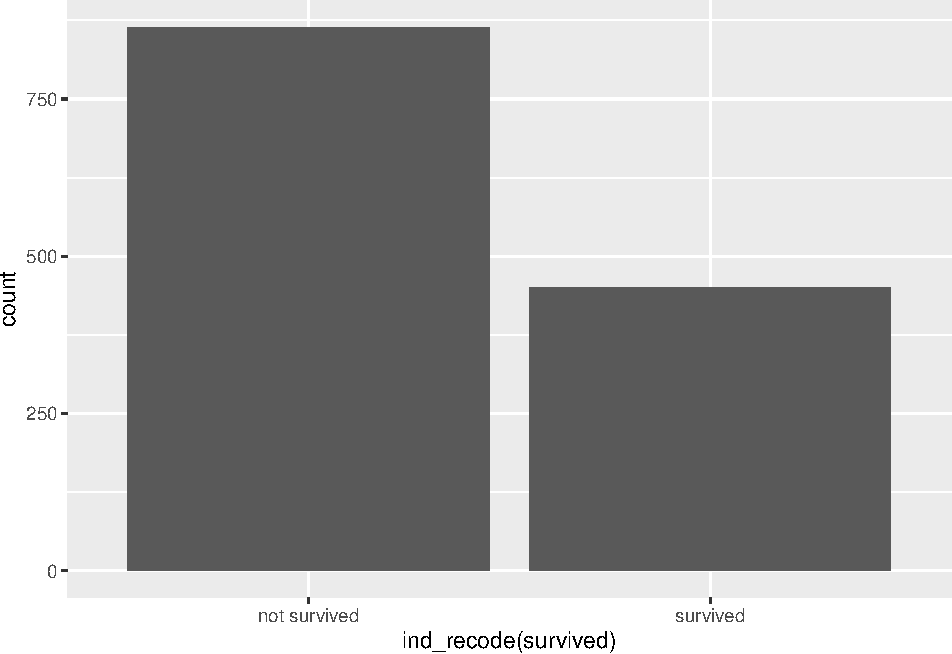
\includegraphics[width=0.69\linewidth]{r_journal_files/figure-latex/unnamed-chunk-13-1} \begin{Sinput}
# or
last_plot() +
  aes(x = ind_recode(survived, cat_false = "perished"))
\end{Sinput}

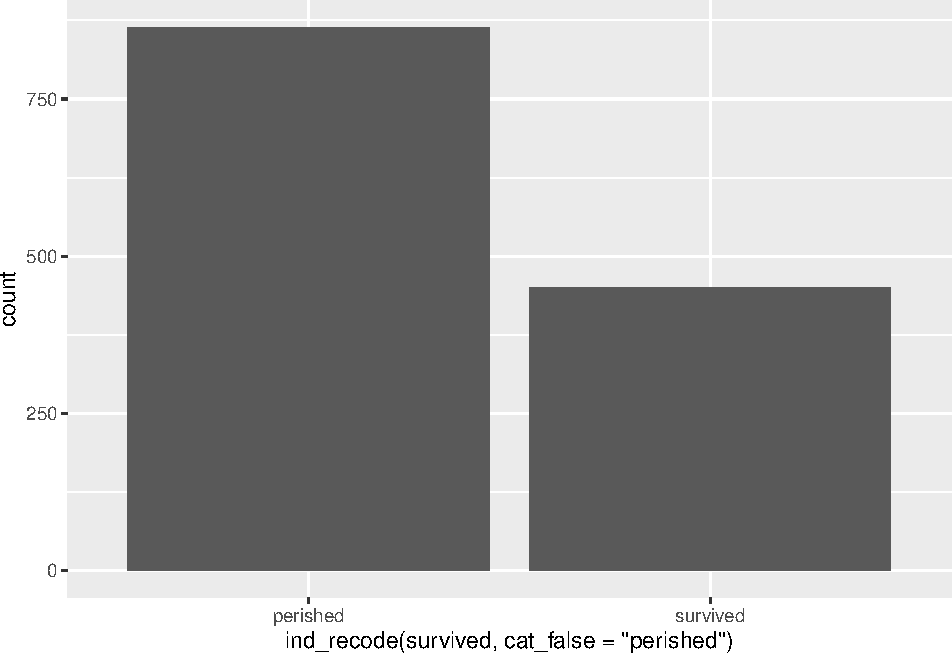
\includegraphics[width=0.69\linewidth]{r_journal_files/figure-latex/unnamed-chunk-13-2} \begin{Sinput}
# or
last_plot() +
  aes(x = ind_recode(survived, cat_false = "didn't", rev = T)) + 
  labs(x = NULL)
\end{Sinput}

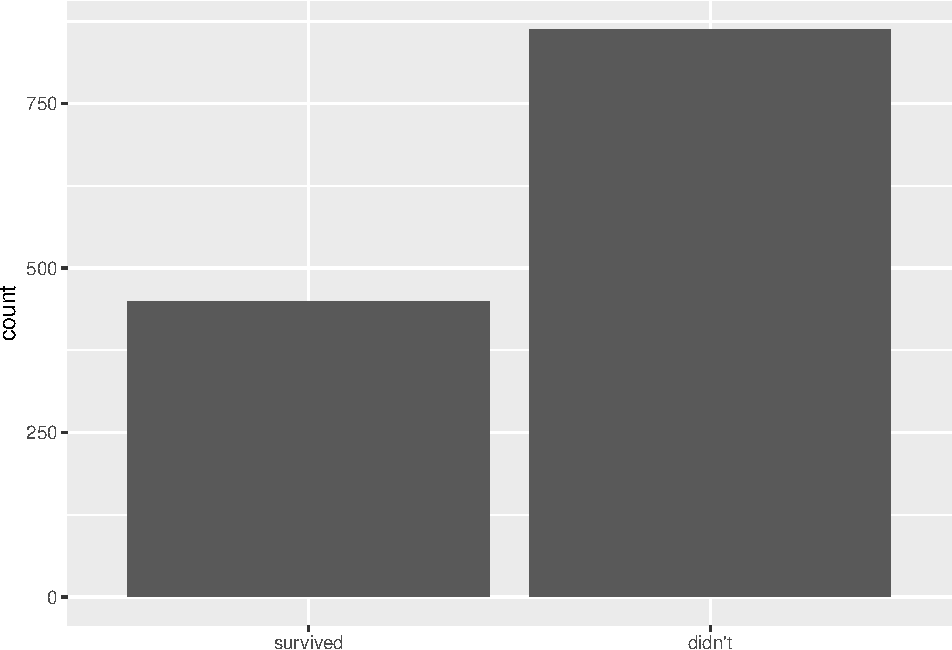
\includegraphics[width=0.69\linewidth]{r_journal_files/figure-latex/unnamed-chunk-13-3} \begin{Sinput}
tidytitanic::passengers %>% 
ggplot() + 
  aes(x = sex) + 
  geom_bar() + 
  facet_grid(~ ind_recode(survived))
\end{Sinput}

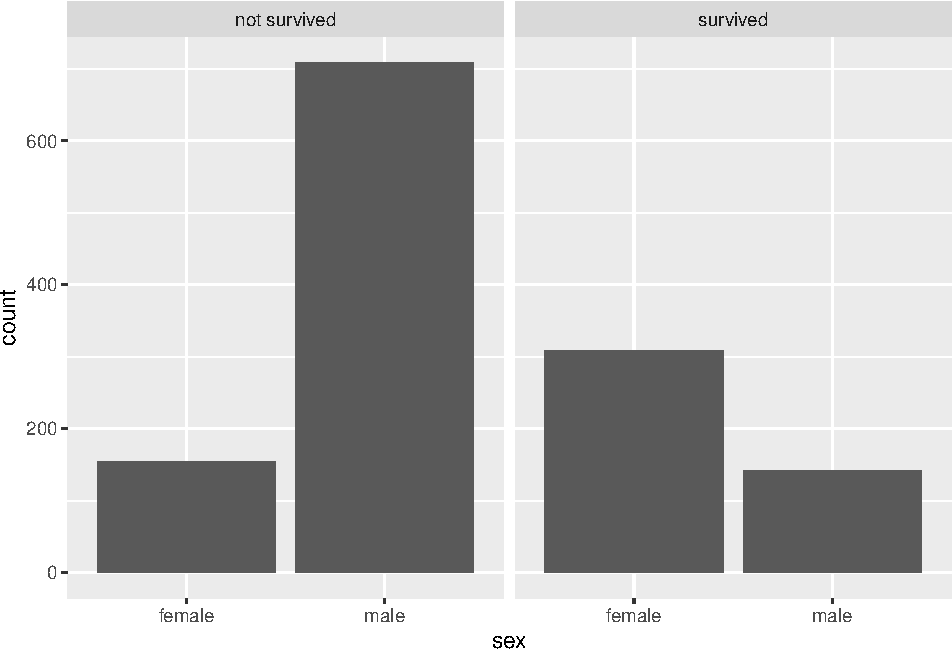
\includegraphics[width=0.69\linewidth]{r_journal_files/figure-latex/unnamed-chunk-13-4} \end{Schunk}

\hypertarget{known-limitations-not-for-use-with-magrittr-pipe-but-base-pipe-works}{%
\section{\texorpdfstring{Known Limitations: \emph{not for use with
magrittr pipe (but base pipe
works!)}}{Known Limitations: not for use with magrittr pipe (but base pipe works!)}}\label{known-limitations-not-for-use-with-magrittr-pipe-but-base-pipe-works}}

\begin{Schunk}
\begin{Sinput}
tidytitanic::passengers %>% 
ggplot() + 
  aes(x = sex) + 
  geom_bar() + 
  facet_grid(~ survived %>% ind_recode())
\end{Sinput}

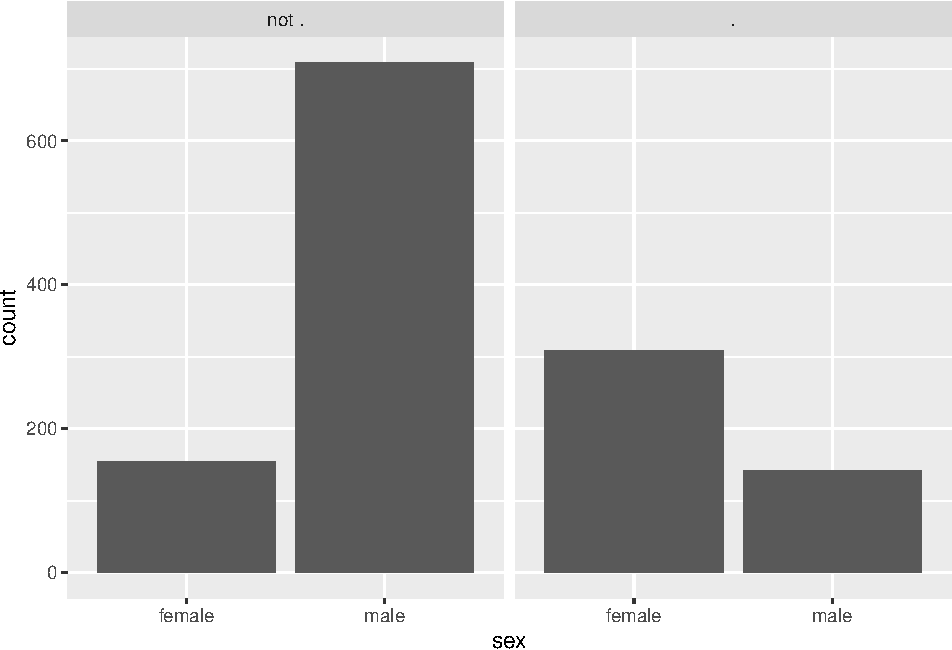
\includegraphics[width=0.69\linewidth]{r_journal_files/figure-latex/unnamed-chunk-14-1} \begin{Sinput}
tidytitanic::passengers %>% 
ggplot() + 
  aes(x = sex) + 
  geom_bar() + 
  facet_grid(~ survived |> ind_recode())
\end{Sinput}

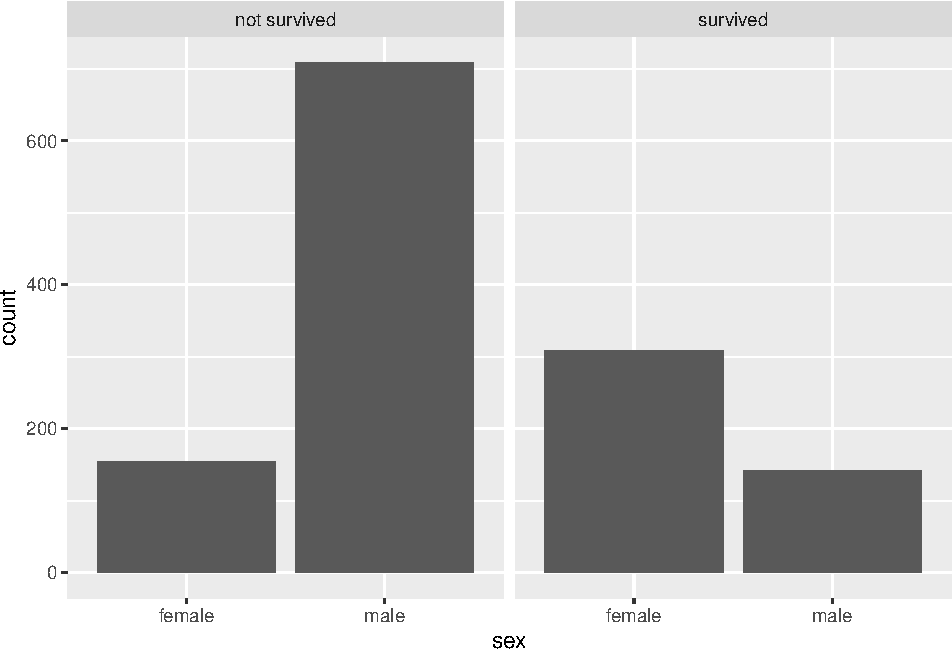
\includegraphics[width=0.69\linewidth]{r_journal_files/figure-latex/unnamed-chunk-14-2} \end{Schunk}

\begin{center}\rule{0.5\linewidth}{0.5pt}\end{center}

\hypertarget{worked-example-with-tidytuesday-data-spam-email}{%
\section{worked example with tidytuesday data, Spam
email}\label{worked-example-with-tidytuesday-data-spam-email}}

\url{https://github.com/rfordatascience/tidytuesday/tree/master/data/2023/2023-08-15}

\begin{Schunk}
\begin{Sinput}
read.csv("https://raw.githubusercontent.com/rfordatascience/tidytuesday/master/data/2023/2023-08-15/spam.csv") %>% 
  rename(spam = yesno) %>% 
  ggplot() + 
  aes(fill = ind_recode(bang>0), x = ind_recode(spam)) + 
  geom_bar(position = "dodge")
\end{Sinput}

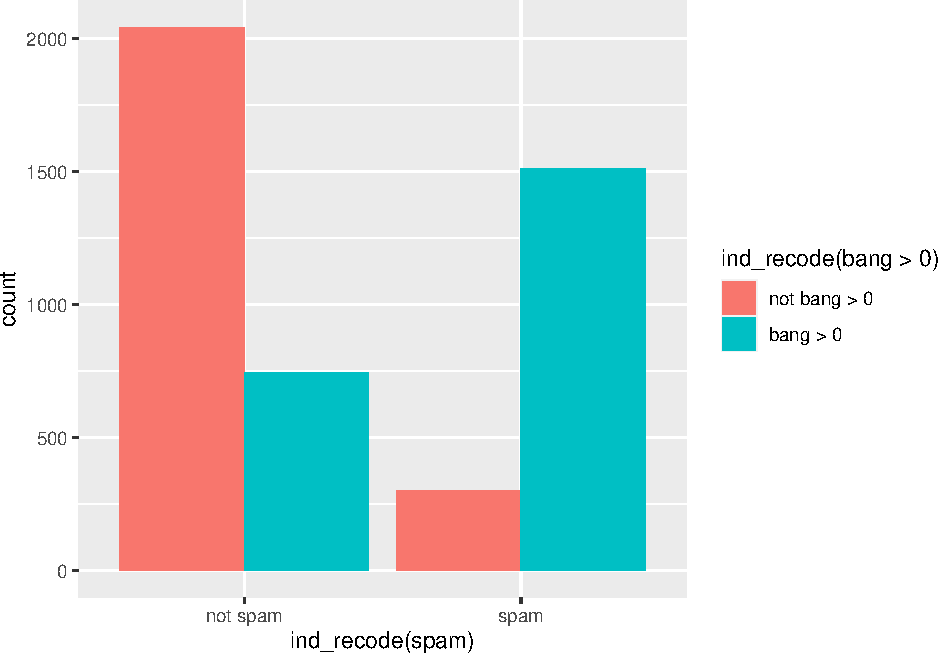
\includegraphics[width=0.69\linewidth]{r_journal_files/figure-latex/unnamed-chunk-15-1} \begin{Sinput}
remove_layers <- function(plot, index = NULL){
  
  if(is.null(index)){
  plot$layers <- NULL
  }else{
  plot$layers[[index]] <- NULL
  }
  
 plot
  
}

last_plot_wiped <- function(index = NULL){
  
  plot <- last_plot()
  
  if(is.null(index)){
  plot$layers <- NULL
  }else{
  plot$layers[[index]] <- NULL
  }
  
 plot
  
}

last_plot_wiped() +
  geom_bar(position = "fill")
\end{Sinput}

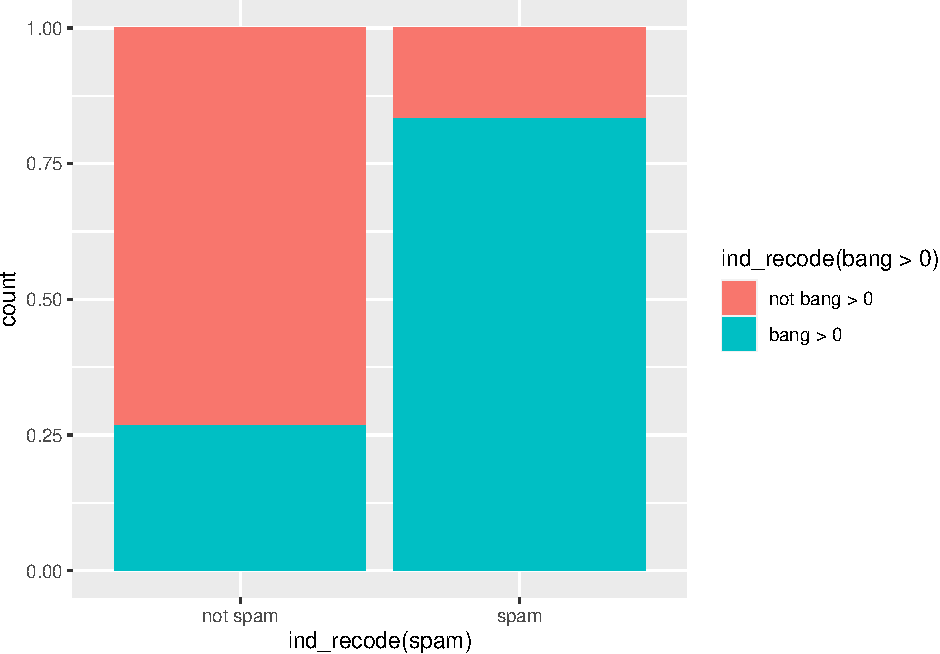
\includegraphics[width=0.69\linewidth]{r_journal_files/figure-latex/unnamed-chunk-15-2} \end{Schunk}

\hypertarget{learned-along-the-way-as_factor-has-different-behavior-than-as.factor}{%
\section{\texorpdfstring{learned along the way: \texttt{as\_factor()}
has different behavior than
\texttt{as.factor()}}{learned along the way: as\_factor() has different behavior than as.factor()}}\label{learned-along-the-way-as_factor-has-different-behavior-than-as.factor}}

\begin{Schunk}
\begin{Sinput}
c("Y", "N") %>% as_factor()
\end{Sinput}
\begin{Soutput}
     [1] Y N
     Levels: Y N
\end{Soutput}
\begin{Sinput}
c("Y", "N") %>% as.factor()
\end{Sinput}
\begin{Soutput}
     [1] Y N
     Levels: N Y
\end{Soutput}
\end{Schunk}

\begin{Schunk}
\begin{Sinput}
# unlink("../../temp.Rmd")
\end{Sinput}
\end{Schunk}

\begin{Schunk}
\begin{Sinput}
rmd_parse <- function(file = "../../README.Rmd"){
  
  readLines(file) %>% 
    data.frame(text = .) %>% 
    dplyr::mutate(ind_section_header = stringr::str_detect(text, "^#"), .before = 1) %>% 
    dplyr::mutate(num_section_level = stringr::str_count(stringr::str_extract(text, "^#+"),"#") ) %>% 
    dplyr::mutate(num_section = cumsum(ind_section_header)) %>% 
    # dplyr::filter(ind_section_header) %>% 
    dplyr::mutate(name_section = ifelse(ind_section_header, text, NA) %>% stringr::str_remove("#+ ") %>% tolower() %>% stringr::str_replace_all("\\s", "_")) ->
  parsed
  
  parsed %>% 
    dplyr::group_by(num_section) %>% 
    dplyr::summarize(text %>% paste0(collapse = "\\n"))
    
  
}
\end{Sinput}
\end{Schunk}

\bibliography{RJreferences.bib}

\address{%
Evangeline Reynolds\\
Affiliation\\%
line 1\\ line 2\\
%
\url{https://journal.r-project.org}\\%
\textit{ORCiD: \href{https://orcid.org/0000-0002-9079-593X}{0000-0002-9079-593X}}\\%
\href{mailto:author1@work}{\nolinkurl{author1@work}}%
}

